\begin{tikzpicture}[x=1cm,y=1cm,scale=0.89,transform shape,
  caso/.style={draw,ellipse,align=center,minimum width=3.6cm,minimum height=0.78cm,font=\scriptsize},
  ator/.style={font=\scriptsize,align=center}]
  \draw (2.5,0.1) rectangle (13.8,6.65);
  \node[anchor=north west,font=\footnotesize\bfseries] at (2.7,6.5) {Estoque Fácil -- administração};
  \node[ator] (adm) at (1.1,3.25) {\begin{tikzpicture}[scale=.55]\draw (0,0) circle (.22);\draw (0,-.22)--(0,-.9) (-.48,-.42)--(.48,-.42) (0,-.9)--(-.42,-1.42) (0,-.9)--(.42,-1.42);\end{tikzpicture}\\Administrador};
  \node[ator] (geral) at (15.25,3.25) {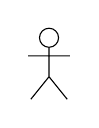
\begin{tikzpicture}[scale=.55]\draw (0,0) circle (.22);\draw (0,-.22)--(0,-.9) (-.48,-.42)--(.48,-.42) (0,-.9)--(-.42,-1.42) (0,-.9)--(.42,-1.42);\end{tikzpicture}\\Administrador geral};
  \node[caso] (cad) at (5.05,5.25) {Manter cadastros\\auxiliares};
  \node[caso] (usu) at (5.05,3.45) {Gerir usuários e perfis};
  \node[caso] (audit) at (5.05,1.65) {Consultar auditoria e logs};
  \node[caso] (emp) at (11.05,5.25) {Gerir empresas clientes};
  \node[caso] (backup) at (11.05,3.45) {Gerar backup};
  \node[caso] (apar) at (11.05,1.65) {Configurar aparência};
  \foreach \n in {cad,usu,audit} \draw (adm.east)--(\n.west);
  \foreach \n in {emp,backup,apar} \draw (geral.west)--(\n.east);
\end{tikzpicture}
